   \begin{abstract}
    Polyploid organisms pose substantial obstacles to genetic analysis, as molecular 
assay data are usually difficult to evaluate in a Mendelian framework. Green sturgeon 
({\em Acipenser medirostris}\/) is a tetraploid species and is facing significant conservation 
challenges, including bycatch in ocean fisheries. We present here novel molecular 
genetic assays and analytical methodology for green sturgeon that allow 
discrimination of fish from the two visually indistinguishable distinct population 
segments (DPSs), and also provide individual-specific genetic tags. We show how 
the relative fluorescence intensity data from a standard quantitative PCR assay, 
designed for a biallelic single nucleotide polymorphism, 
can be grouped into ``genotype categories'' using 
standard analytical software and post-processing manipulation. We then show how 
these genotype category data can be used to discriminate green sturgeon from the 
southern DPS, which is protected under the US Endangered Species Act, and the 
northern DPS, which is not. We also show how these data can be used to reliably 
identify individual green sturgeon, and can therefore be used in capture/recapture 
analyses. Both types of identification are extremely accurate even when fewer than 
half of the assays are successfully called. We then apply these new techniques to 
show that proportions of the two green sturgeon DPSs are extremely different in the 
two major fishery areas where they are encountered as bycatch. While these assays 
and methods do not provide data that can be used in pedigree-based analyses, they 
are an important advance in the application of genetic analysis to conservation and 
management of polyploid organisms.	
   \end{abstract}
%%%%%%%%%%%%%%%% START MAIN BODY

\section{Introduction}

Polyploidy, the presence of more than two copies of the genome in an individual,
is relatively common in plants and invertebrates, but uncommon in vertebrates~\citep{Mable2004}. 
Sturgeon, fishes in the family {\em Acipenseridae}, have a number of species that are 
polyploid and the mosaic of ploidy in the group suggests a polyploid ancestor, 
with subsequent rediploidization in some species and further genome duplication 
in others~\citep{ludwig2001genome}, although high homology between genome copies in 
some species contradicts the polyploid ancestor hypothesis \citep{havelka2011sturgeon}. While 
the causes of this unusually high prevalence of polyploidy in sturgeon remain 
to be elucidated, its consequences for molecular population genetics are clear: 
the presence of more than two copies of each gene region greatly complicates 
use of molecular genetic data in all methods that make an assumption of Mendelian segregation.

We describe here novel molecular genetic markers and methodology for the study
of 
one such polyploid fish species, green sturgeon ({\em Acipenser medirostris}). Green sturgeon are anadromous fish
inhabiting the northeastern Pacific and its tributaries. Spawning activity is
known to occur primarily in the Sacramento, Klamath and Rogue river basins
\citep{adams2007population}, although adult green sturgeon enter other rivers and evidence of
spawning activity has recently been observed in the the Columbia River (Ethan Mora, pers.\ comm.) and
in the Eel River of California~(J.~Strange and S.~Kullman, pers.\ comm.)

Previous status reviews \citep{adams2007population,nmfs2015sturgeon} have determined that
there are two Distinct Population Segments (DPSs) of green sturgeon. The
Southern Green Sturgeon DPS includes fish originating from the Sacramento River,
and the Northern Green Sturgeon DPS includes fish originating from the Klamath
and Rogue rivers. Previous evaluations \citep{adams2007population,nmfs2015sturgeon} have
determined that the Southern DPS is threatened with risk of extinction and it
has been listed for protection as such under the US Endangered Species Act (ESA). The
Northern DPS is a National Marine Fisheries Service (NMFS) Species of Concern.

Effective conservation and management of green sturgeon requires identifying 
fish from these visually indistinguishable DPSs when they are encountered in 
ocean fisheries and elsewhere and we describe the development of genetic 
assays and analytical methodology that allow such identification. Specifically, 
we have used next generation (high-throughput)
DNA sequencing to identify variable sites (variants) in the green sturgeon
genome and used this information to develop a panel of molecular assays that
target those sites and can be used to characterize these variants in
individual fish. The initial application goal for these genetic markers was to
use them in identifying individual fish to their DPS of origin. The
secondary objective was to evaluate their ability to identify specific
individuals that have been sampled more than once (i.e., as DNA ``fingerprints'').

Green sturgeon are not only tetraploid but they appear to have experienced a 
recent duplication of their entire genome, with very high homology of 
the different genome copies~\citep{Israeletal2009}. As such, they are not amenable to traditional
population genetic evaluation using the methods developed for calling genotypes
in diploid species, since designating alleles to genome 
copies is nearly impossible. 
We have therefore developed a genotyping system and workflow to allow 
calling of such variants in tetraploid species. 
This methodology uses quantitative PCR assay data 
but does not call the individual alleles and the dosage 
(number of copies) carried by each tetraploid individual, but, rather, 
places individuals into ``genotype categories.''  The
inheritance properties of such genotype categories are not directly considered
in the statistical analysis, but the data are still suitable for both the assignment
of individuals to DPS and the identification of samples from the same
individual.

We describe below how these new markers and methods uncover a substantial amount
of genetic differentiation between the two green sturgeon DPSs, and that the
panel of SNP markers and the statistical procedures we have developed provide a
robust, cost-effective, and extremely accurate means of identifying the DPS of
origin for individual green sturgeon and of identifying green sturgeon that have
been sampled multiple times. We then use genetic assay data from green sturgeon
caught as bycatch in ocean fisheries off the west coast of North America to start
to elucidate population-specific patterns of ocean distribution. We also identify
the DPS of origin of fish that apparently represent a recolonization of part of the species
historic reproductive range. The analytical methodology we describe, assigning genotype
categories rather than calling specific genotypes that have an assumption of 
Mendelian segregation, has broad relevance to the study of polyploid species 
and will allow biological inference regarding identity at the population and 
individual level to be derived from standard SNP genotyping assay data.








%%%%% HERE ARE THOUGHTS FOR AN INTRODUCTION FOR A JOURNAL PAPER  %%%%%%%%%%%
% This is super free-form, stream of consciousnessy at the moment, as I get some ideas
% down onto the page.
% 
% The study of highly migratory species in environments that are difficult to monitor present
% a number of challenges.   Often, the migrations themselves cannot be observed.
% Genetic data has been successful in inferring the ecology of a number of species
% that are otherwise difficult to study (CITE).  It is now fairly routine to do this
% in most species, especially diploid ones.  Genetic methodologies are well-established for microsats, SNPs, and to an increasing extent, lately, next generation sequencing data.
% Concurrently, the last two decades have seen an explosion in the availability statistical
% methods for analyzing genetic data.  
% 
% The vast majority of methods have been developed for diploid organisms.  When these methods
% can be extended to polyploids their extension
% typically requires that the number of copies of individual alleles can be resolved in a
% polyploid genotype, or that the exact inheritance patterns are known, which is not always
% the case.  The challenges of polyploids have been
% well-appreciated in botanical fields for some time (CITE Fisher's polyploid inheritance
% paper), and these difficulties have been gaining increasing attention in the field of
% molecular ecology (CITE that recent review).  
% 
% Significant advances have been made in the development of models for polyploids and
% particularly for tetraploids, for example, fitTetra, and the work from Brazil on
% sugar cane.  However, sometimes that quality of scoring is not high enough to 
% resolve all those allele copies. Furthermore, the assumptions underylying fitTetra
% are probably not appropriate when samples are mixture of diverged tetraploid populations.
% (ERIC VERIFY THIS)
% Clearly, it would be best to be able to resolve
% and count all the alleles, but in cases where that is not possible for a majority of the
% loci that have been discovered, alternative modes of analysis are sought.  One such
% alternative analysis method is to treat alleles in polyploids as dominant markers.  This
% approach has been used recently in population assignment (Israel et al.) and CITE, and CITE,
% and more recently Wang and Scribner have shown the utility of that approach for doing
% relationship inference.  
% 
% Modeling everything as a dominant marker (presence/absence of the allele) is particularly
% well-suited to microsatellite loci where length polymorphisms are easy to interpret.
% However, using xxxxxx-type SNP assays (like fluidigm assays)  the individual alleles
% may not be so easily resolved, because the scoring relies on individual genotypes clustering
% in two space, and it might not always be easy to resolve the 5 expected genotype clusters.
% For such data, trying to resolve the data into individual, expected genotype categories
% might be unworkable for many loci, especially if typing members of fairly well-diverged
% lineages.  Depending on the goal of genetic analysis, however, it may still not be
% necessary to require thinking about the data only as  individual alleles giving rise to
% a full complement of expected genotypes.
%%%%%%%%%%%%%%%%%%%%%%%%%%%%%%%%%%%%%%%%%%%%%


\section{Methods}



\subsection{Genetic Samples}

We analyzed samples of three general categories. The first is from fish sampled in
two rivers known to have well-established spawning populations of green
sturgeon---the Sacramento River and the Klamath River. These samples were used to
construct the ``reference'' or ``baseline'' dataset. All of these samples were taken
from juvenile fish or from eggs collected on egg mats, either of which must have
been spawned (originated) in the river from which they were sampled. We refer to
these as ``egg/juvenile reference'' samples. There were also a few samples taken
from adult or sub-adult fish in the Sacramento River that may be non-spawning
visitors, originating in a different river, and these are referred to as
``non-juvenile reference'' samples. Samples taken from the ocean or from rivers
without a persistent spawning population are ``non-reference''
samples. These include green sturgeon caught as bycatch in ocean fisheries, and
five fish sampled from the Eel River, CA. See Table~\ref{tab:samps} for a summary of sample
types and sample sizes. 
\begin{table*}
\caption{Summary of genetic samples used in this study.}
\begin{center}
\begin{tabular}{llllr}
\hline \hline \\ 
Location & Category & Life Stage & Group Short Name & n & Collection Years\\ \hline
Sacramento River & reference & egg & reSac & 66 & 2011--2012\\
Sacramento River & reference & juvenile & rjSac & 72 & 2012--2013\\
Sacramento River & reference & non-juvenile & rnSac & 12 & 2014\\
Klamath River & reference & juvenile & rjKla & 21 & 2006\\
Eel River & non-reference & non-juvenile & nnEel & 5 & 2015\\
Bycatch & non-reference & non-juvenile & nnByc & 190 & 2008--2014\\

\hline \hline \\ 
\end{tabular}
\end{center}
\label{tab:samps}
\end{table*}
Tissue samples were of various types, including fin clips, either dried or 
stored in ethanol, and whole eggs or whole
juvenile specimens stored in ethanol.


\subsection{SNP Discovery and Assay Development}

To identify SNPs to be made into assays, we first collected DNA sequence
information from eight green sturgeon, four juveniles from the Klamath River 
(Northern DPS) and four juveniles from the Sacramento River (Southern DPS). 
These are referred to as the ``ascertainment'' samples. We used a double-digest restriction-site associated
DNA protocol (ddRAD; \citealt{Petersonetal2012}), which uses restriction
enzyme digestion and DNA fragment size selection to reduce the fraction of the
genome that is analyzed, ensuring that a sufficiently small portion is
sequenced to provide adequate numbers of DNA sequences (read depth) from the
eight different individuals. DNA sequencing was on a MiSeq DNA sequencer 
(Illumina Inc., San Diego, CA) and yielded 21.24 million sequence reads, 
each of 300 bp in length. We used Stacks software v 1.12 \citep{catchen2011stacks} 
under the following parameter settings---$m = 4$, $M = 2$, $n = 2$---to assemble 
the sequences into 84,747 putatively unique genetic loci. Within those loci, 
we identified 21,218 SNPs with minor allele frequencies greater than 0.25 
in the sample of eight fish. At 1,118 of the SNPs, the four Klamath fish 
had a single variant that was different from the single variant carried by 
the four Sacramento fish. Of these 1,118 SNPs, we chose 96 with the highest 
read depths and quality scores for \snptype{} genotyping assay design 
(Fluidigm Co., South San Francisco, CA). Although these SNPs appeared
to be fixed for alternate variants in the ascertainment samples from the 
two DPSs, many of them were polymorphic in the large set of reference samples (see Results).

The 96 assays were then validated on 96.96 SNP Genotyping Arrays (Fluidigm) 
which use nanofluidic technology to simultaneously genotype all 9,216 
combinations of 96 assays and 96 individuals on a single array (hereafter called “chip”). 
These assays contain two gene probes that are specific to the two variants 
uncovered in the next generation sequencing effort. These probes carry 
fluorescent dyes that measure the relative abundance of the two variants 
and report them as relative fluorescence intensities in a two-dimensional 
coordinate space. Each variant at a SNP therefore corresponds to a 
fluorescent dye and the genotype of a diploid individual can be called 
from the intensity of fluorescence for each of those dyes. 
Fluidigm provides software that allows genotype calling of diploid 
individuals, but the software is not designed for the calling of tetraploid genotypes. 


\subsection{Developing Calling Methodology}
Apparent in our data were two difficult features. First, data from most of the green sturgeon SNP
assays did not consist of five clearly callable
fluorescence clusters (genotypes), as expected for tetraploids; rather, many of
the clusters in the fluorescence intensity data were indistinct or overlapping.
Second, we encountered considerable chip-to-chip variation in fluorescence
intensity. To deal with the indistinct clustering, it suffices to put an
individual into a particular {\em genotype category} without reference to the
underlying alleles. In this scheme, individuals with different {\em genotypes} may be put in the
same genotype {\em category} if the genotypes are difficult to resolve on
the basis of their fluorescence intensities. To address the chip- to-chip
variation, each chip includes samples from a number of individuals that have
been previously analyzed, so that corresponding clusters between the chips can
be identified and the corresponding fluorescence intensities used to calibrate calling across chips.

We first used four chips to decide which loci were consistently callable 
({\em call-development chips}) and, at each locus, the number of genotype categories that
could be resolved. Some individuals were genotyped on multiple chips to evaluate chip-to-chip variation (Table~\ref{tab:devo-samps}). 
%%%%%%%%%%%%%%%
\begin{table}
\hrule \kern 0.5mm \hrule
\small
\caption{Four scoring-development chips}
\label{tab:devo-samps}
(a) Number of samples from each location
\begin{center}
\begin{tabular}{lrrr}
Chip & Sacramento & Klamath & Bycatch\\\hline
1 & 0 & 17 & 77\\
2 & 54 & 17 & 23\\
3 & 78 & 8 & 8\\
4 & 37 & 2 & 55\\

\hline
\end{tabular}
\end{center}
\mbox{}\\
(b) Number of samples shared between chips
\begin{center}
\begin{tabular}{lrrrr}
Chip & 1 & 2 & 3 & 4\\\hline
1 & 94 & 13 & 6 & 9\\
2 &  & 94 & 8 & 4\\
3 &  &  & 94 & 32\\
4 &  &  &  & 94\\

\hline
\end{tabular}
\end{center}
\hrule
\end{table}
%%%%%%%%%%%%%%%%%%%%%
We then created a
series of graphs (one for each locus) that plotted the raw fluorescence
intensities from the Fluidigm chip reader~(Figure~\ref{fig:plate_xy}). The {\em raw} intensities
were not transformed based on the
observed intensity of the two no-template controls (NTCs) that are included on every chip.
%Raw intensities are not available from the
%Fluidigm SNP Genotyping Analysis Software by default, but, with a request and a code from
%Fluidigm technical support (ph.~866-358-4354), they can be accessed.  
We used the raw intensities because there was less chip-to-chip
variability in them
compared to the default NTC-normalized values from the Fluidigm software. On these 
graphs, results from each
chip are in a different color and points for the same sample genotyped on
different chips are connected with line segments. The plots of four exemplar loci
with 2--5 genotype categories regarded as callable are
shown (Figure~\ref{fig:plate_xy}). 
Similar plots for all of the loci are in the Supplemental Figures.
\begin{figure*}
(a)\\
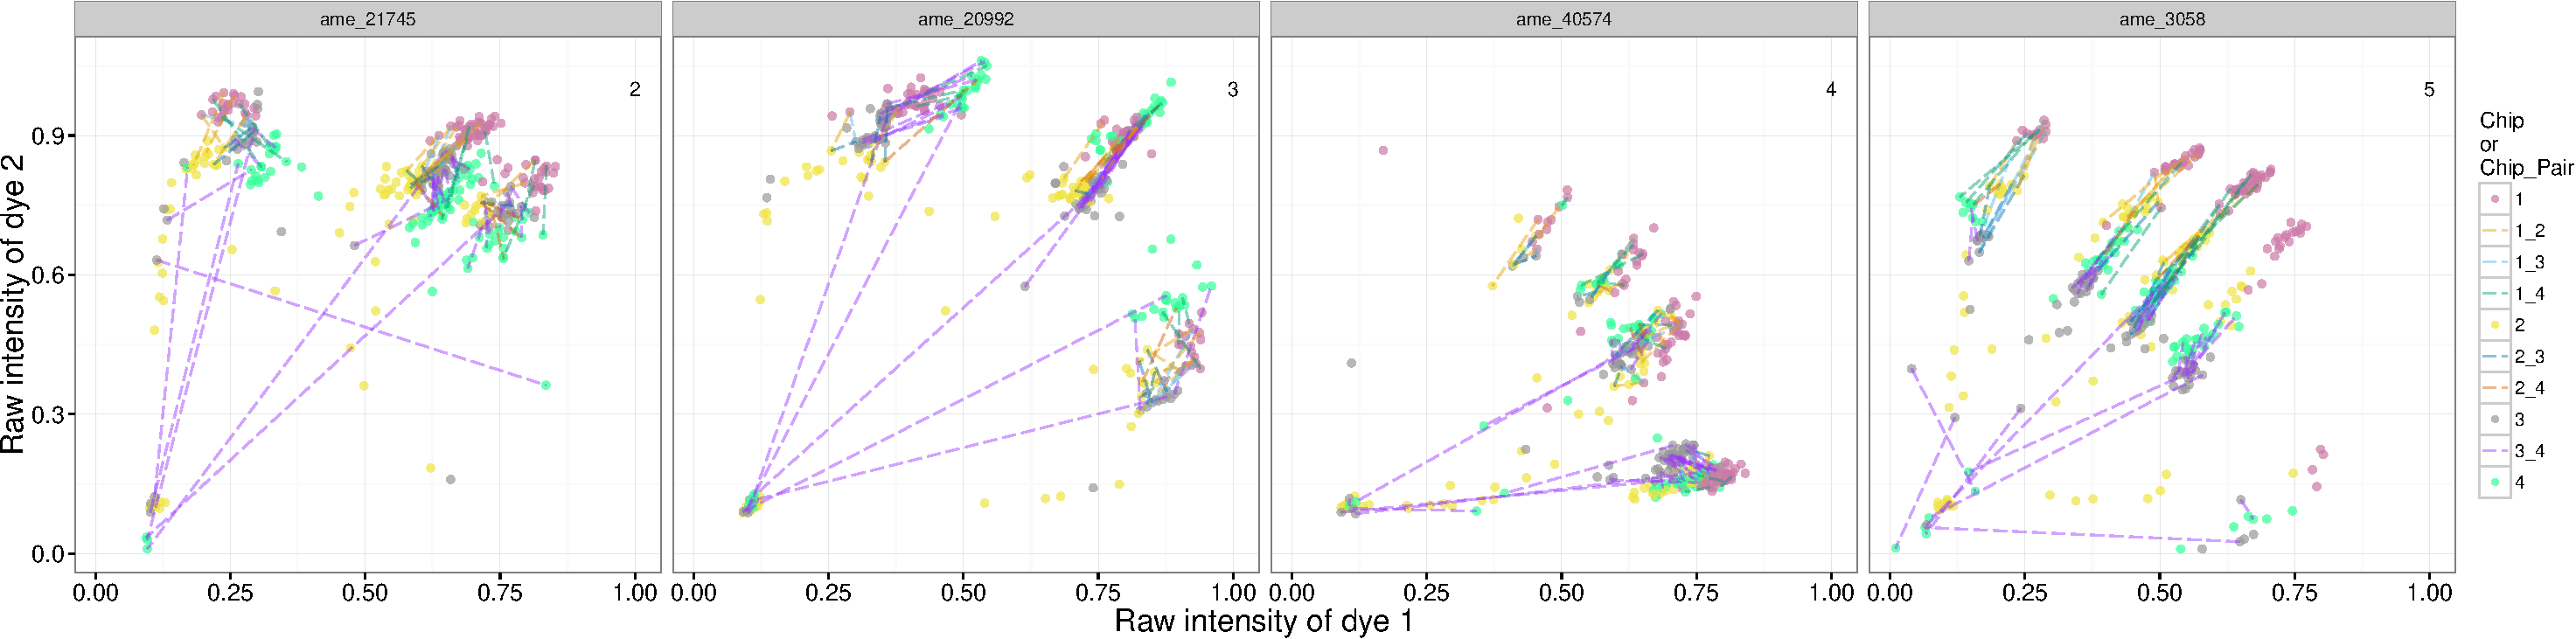
\includegraphics[width = \textwidth]{inputs/four_loci_by_plate-crop.pdf} \\
(b)\\
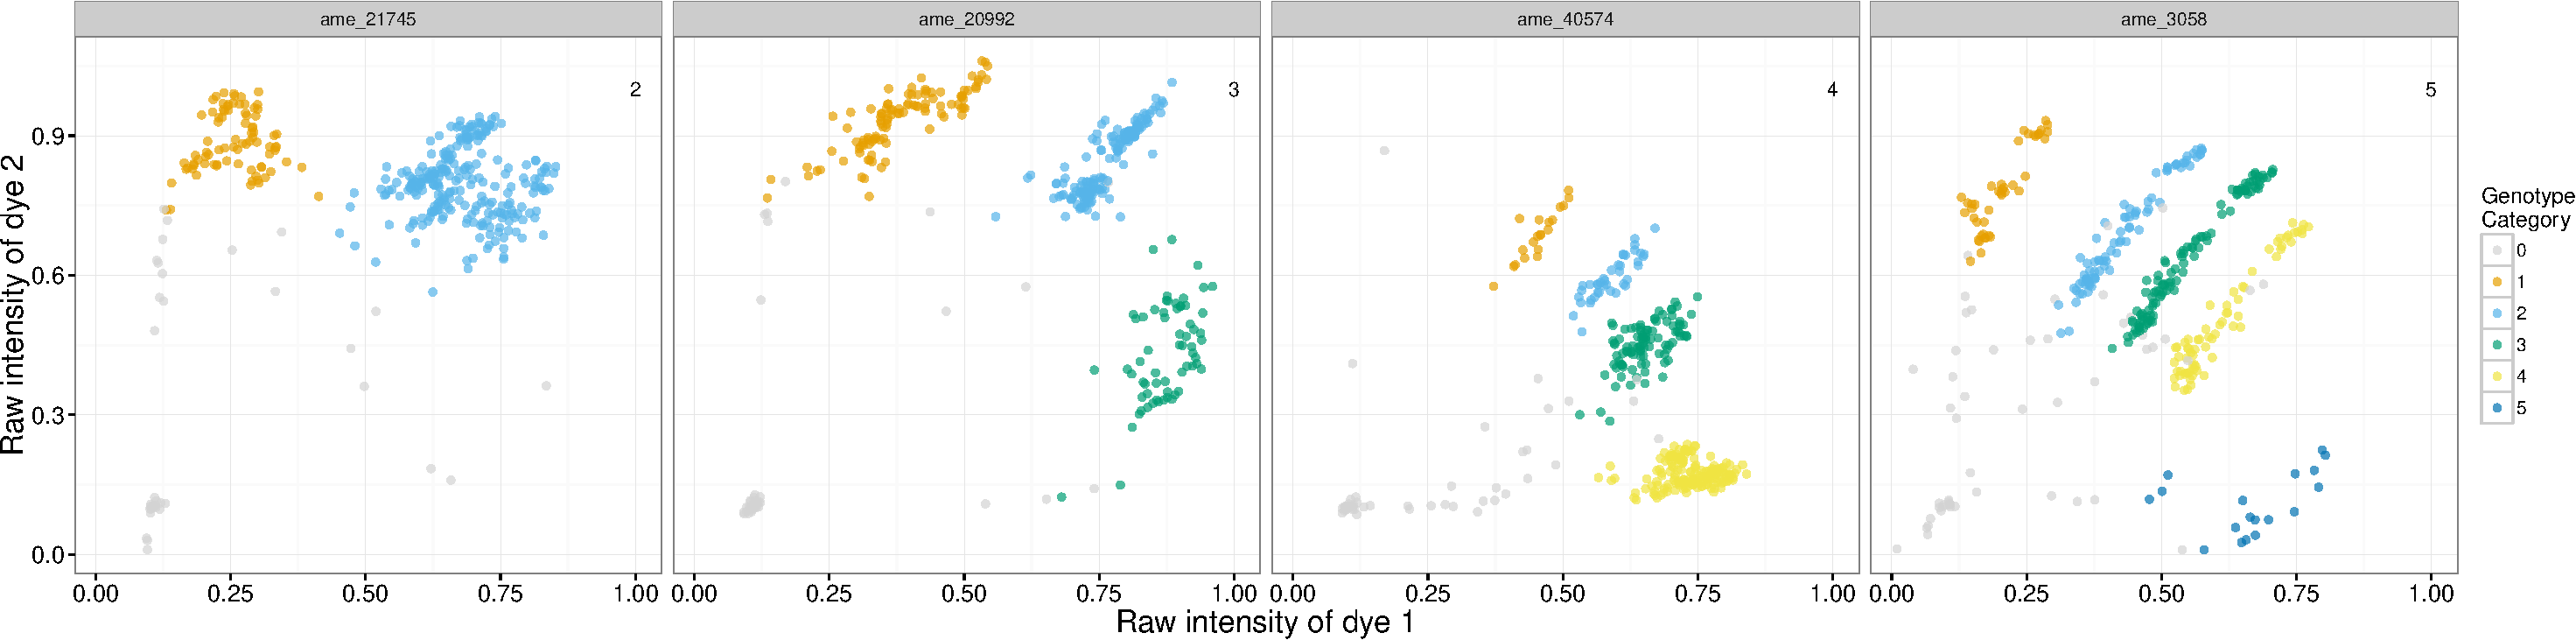
\includegraphics[width = \textwidth]{inputs/four_loci_by_geno-crop.pdf}
\caption{ Raw \snptype{} fluorescence intensities at four loci typed upon the four
scoring-development chips. Each panel
shows the results at four chips for one locus.  The numeral in the upper right gives the number
of genotype categories that are scored at the locus.  Each point represents an individual's fluorescence
intensities at two dyes. ({\em a}) Individuals are colored according to chip and dashed line
segments connect the intensities of individuals typed on different chips. ({\em b}) Individuals are colored
according to the genotype category to which they have been scored.  Category~0 (colored light gray) is a ``no call'', \ie the individual
is recorded as having missing data at the locus. The Supplemental Figures contain plots 
like these for all 96 assays.}
\label{fig:plate_xy}
\end{figure*}
In general, we preferred to merge
nearby clusters into a single genotype category, ensuring that genotype
categories could be called reliably, rather than maintaining 
more genotype
categories, some of which could be subject to high rates of
categorization error. For example, at 
locus ame\_21745 (Figure~\ref{fig:plate_xy}{\em a})    
there are three clusters apparent, but two  
are rather close together and could be difficult to resolve in the face of
substantial chip-to-chip variation.   Accordingly,
we choose to call only two genotype categories for this locus.

For subsequent chips we followed a simple routine. First, we included between 16
and 24 individuals from the call-development chips on each new chip. Second, we
plotted the raw fluorescence intensities of the new chip along with the raw
intensities of the four call-development chips, including line segments
connecting the results from the 16 to 24 individuals on the old and the new
chips to verify the correspondence between clusters. 
We then analyzed the new chip using the Fluidigm SNP Genotyping
software which allows the user to call up to three clusters of 
fluorescence intensity. Because
this software allows genotypes to be called into only three categories (as
expected for a SNP locus with two alleles in a diploid species), we called genotypes
into these three allowed categories and used a custom R script \citep{RCore2015} 
to convert those calls into up to five categories by using
a combination of the genotype calls and the fluorescence intensities. As
an example, when we designate a genotype in the Fluidigm software as a~`1'---a homozygote that typically clusters
in the lower right part of the X-Y plot of fluorescent intensity---but its
intensities are such that it falls in the upper left part of the X-Y plot, then,
we convert that call to genotype category `4'. If the point fell in
the lower right part of the plot, then it would have remained in genotype
category `1'.  To ensure that this combined calling procedure, with initial
Fluidigm software analysis followed by post-processing adjustment
to resolve the five genotype categories, can be done easily by others, our 
entire workflow is available and documented at \url{https://github.com/ngthomas/sturgeon_fluidigm}.



\subsection{Population structure,  population assignment, and individual assignment}

Our calling method does not resolve the exact genotype of each individual. That is, the
precise number of copies of each different allele within an individual is not
obtained. Accordingly, these data are not appropriate for use with analytical
methods that assume Mendelian segregation or information about the individual, 
constituent alleles of each
individual's genotype. However, it is still valid to apply 
a number of statistical analyses, including the model-based clustering method
in the program {\em structure} by assuming haploid inheritance for each genotype category,
and using the model without admixture. 
In this case, the software implements a finite mixture model in which 
the component-specific parameters are the frequencies of different genotype categories
at each locus, and an individual's genotype category is assumed drawn, independently 
at each locus, from these frequencies.  
Such a model does not require any assumptions about
constituent alleles or the mode of their inheritance.
We included all individuals from which we had successfully
obtained calls at 60 or more assays in an analysis with {\em structure} at $K$ (the number
of genetic groups or populations) equal to one, two, and three, running it
multiple times at each $K$. We used no prior information about the origin
of the reference samples. Our aim was to evaluate the genetic clustering of
individuals from the ``reference'' sample collections and whether they
consistently grouped into two clusters, coincident with the DPS categorization.

Similarly, population assignment or, as it is often called in
fisheries, ``genetic stock identification'' (GSI), can be carried out under a
haploid model, using our definition of genotype categories. The model underlying
GSI is nearly identical to the ``without admixture`` model of {\em structure}, except that 1)
{\em structure} assumes that the proportion of individuals from each component is
equal, while in GSI that proportion is estimated, and 2) {\em structure}
can perform unsupervised clustering, while for GSI, known samples from each
DPS are used as ``baseline'' samples. We used the reference samples from the Sacramento and
Klamath rivers as our baseline samples from the Southern and Northern DPSs,
respectively. We assessed accuracy of self-assignment of the
baseline samples using a leave-one-out procedure, and then we performed GSI on
the remaining samples (fishery bycatch and Eel River samples), using the
expectation-maximization algorithm \citep{Dempsteretal1977} to maximize the likelihood. All analyses
were done using the software {\em gsi\_sim} \citep{Andersonetal2008,Israeletal2009}, 
which returns an estimate of the posterior probability that each fish
belongs to the Southern or Northern DPS.

We also 
investigated whether the observed genotype
categories can be used to identify the same individual when it is sampled more than once.
For this purpose, we developed a straightforward log-likelihood ratio statistic
to discriminate genotypes from samples taken from the same individual
green sturgeon and those taken from different individuals. We compared the
distribution of the statistic in both simulated and observed genetic
assay data from pairs of samples known to be from the same fish, 
both from DNA samples subjected to genotyping more than once and from
independent DNA extractions from tissue taken from the same individual.

To derive our log-likelihood ratio statistic, let $\bp_\ell$ 
be the frequencies of the genotype categories at locus $\ell$ in the DPS from which a pair of individuals
originate.  For example, if four categories are 
scored at locus $\ell$, then $\bp = (p_{\ell,1}, \ldots, p_{\ell,4})$, with $\sum_{k=1}^4 p_{\ell,k} = 1$.
Assume that at locus $\ell$ a fraction $\epsilon_\ell$ of the samples is expected to be subject to 
genotyping error.  If a sample is subject to genotyping error, then its observed genotype category
is drawn from $\bp_\ell$, independently of its true, unobserved genotype category. Though this is
a somewhat unrealistic genotyping error model, it is mathematically convenient and adequate for
our purposes.  Under this assumption,
the marginal probability that a sample, $i$, is observed to have genotype category $g$ at locus $\ell$ is
\[
P(y^{(i)}_\ell = g) = (1-\epsilon)p_{\ell,g} + \epsilon p_{\ell,g} = p_{\ell,g}.
\]
If another sample $j$ that is unrelated to sample $i$---we shall say $K_{ij} = \mathrm{U}$---is typed
and found to have genotype category $h$ (which may be the same category as $g$) then the joint probability is simply
\begin{eqnarray}
P(y^{(i)}_\ell = g, y^{(i)}_\ell = h | K_{ij} = \mathrm{U}) &=& P(y^{(i)}_\ell = g)P(y^{(j)}_\ell = h)  \nonumber \\
& = & p_{\ell,g} p_{\ell,h}  \label{eq:pairU}
\end{eqnarray}
If $i$ and $j$ are two samples from the same individual ($K_{ij} = \mathrm{S}$), then the joint probability of the observed genotypes
can be written as a sum over the four possible cases: 1) neither sample suffered a genotyping error; 2) $i$ suffered
an error, but not $j$; 3) $j$ suffered an error, but not $i$; or 4) both $i$ and $j$ suffered an error:
\begin{eqnarray*}
\lefteqn{P(y^{(i)}_\ell = g, y^{(i)}_\ell = h | K_{ij} = \mathrm{S})  =} \\
& & (1-\epsilon_\ell)^2  p_{\ell,g}  \delta(g = h)  \\
& & \mbox{} + \epsilon_\ell p_{\ell,g} \times (1-\epsilon_\ell) p_{\ell,h}  \\
& & \mbox{} + (1-\epsilon_\ell)p_{\ell,g} \times \epsilon_\ell p_{\ell,h} \\
& & \mbox{} + \epsilon_\ell^2 p_{\ell,g} p_{\ell,h},
\end{eqnarray*}
where $\delta(g = h)$ is 1 when $g=h$ and 0 otherwise.  This can be written more compactly as
\begin{eqnarray}
\lefteqn{P(y^{(i)}_\ell = g, y^{(i)}_\ell = h | K_{ij} = \mathrm{S})  =} \\ \nonumber
& & (1-\epsilon_\ell)^2  p_{\ell,g}  \delta(g = h) + (2\epsilon_\ell - \epsilon_\ell^2) p_{\ell,g} p_{\ell,h}. \label{eq:pairS}
\end{eqnarray}

A log-likelihood ratio statistic that can be used to
identify pairs of samples $i$ and $j$ from the same
individual is then
\begin{equation}
\Lambda_{ij}= \log\frac{P(y^{(i)}_\ell = g, y^{(i)}_\ell = h | K_{ij} = \mathrm{S})}
{P(y^{(i)}_\ell = g, y^{(i)}_\ell = h | K_{ij} = \mathrm{U})}.
\label{eq:logl}
\end{equation}
To approximate the distribution of
$\Lambda_{ij}$ under $K_{ij} = \mathrm{S}$ and $K_{ij} = \mathrm{U}$, we
conducted Monte Carlo simulations using values of $\bp$ for the Northern and Southern DPSs obtained
by counting genotyping categories scored on individuals assigned by {\em structure} to
the Northern DPS and Southern DPS
clusters.  For the simulation of pairs and for the calculation
of $P(y^{(i)}_\ell = g, y^{(i)}_\ell = h | K_{ij} = \mathrm{S}$) 
for each simulated pair, we assumed a conservatively high genotyping error rate of
$\epsilon_\ell = 0.05$ for every locus.  
$10^5$ genotype pairs were simulated both for $K_{ij} = \mathrm{S}$ and $K_{ij} = \mathrm{U}$.
Simulations were first done for 
the case in which every pair was scored at all of the SNPs developed in our
panel. Then, to investigate the expected
distributions when pairs shared fewer scored loci due to missing data (\ie loci that were not scored),
we successively deleted loci randomly, without replacement, according to 
the observed locus-specific missing
data rates in our data set, from each simulated pair, and recomputed the $\Lambda_{ij}$ values.
We computed $\Lambda_{ij}$ for all pairs
$ij$ of fish from amongst those assigned by {\em structure} to the
Northern DPS or the Southern DPS\@. Both the
simulations and the pairwise comparisons of real fish were done using a custom-written
script in R \citep{RCore2015}.

\section{Results}

\subsection{Loci scored}

Of the 96 SNP assays developed, 74 of them could be reliably called into
genotype categories (Supplemental Table~1).  Of these, 39 were loci with two 
categories, 29 with
three, 3 with four, and 3 with five. Of the 470 total DNA samples analyzed with
these SNP assays, 413 (corresponding to 319 distinct green sturgeon, since some
were genotyped more than once) yielded called genotype categories for at least 60
of the 74 loci. Inspection of the distribution of the number of called loci
revealed that only the egg samples from the Sacramento River consistently failed
to genotype well ($<$60 called assays; Figure~\ref{fig:success-histos}).

\begin{figure}
\begin{center}
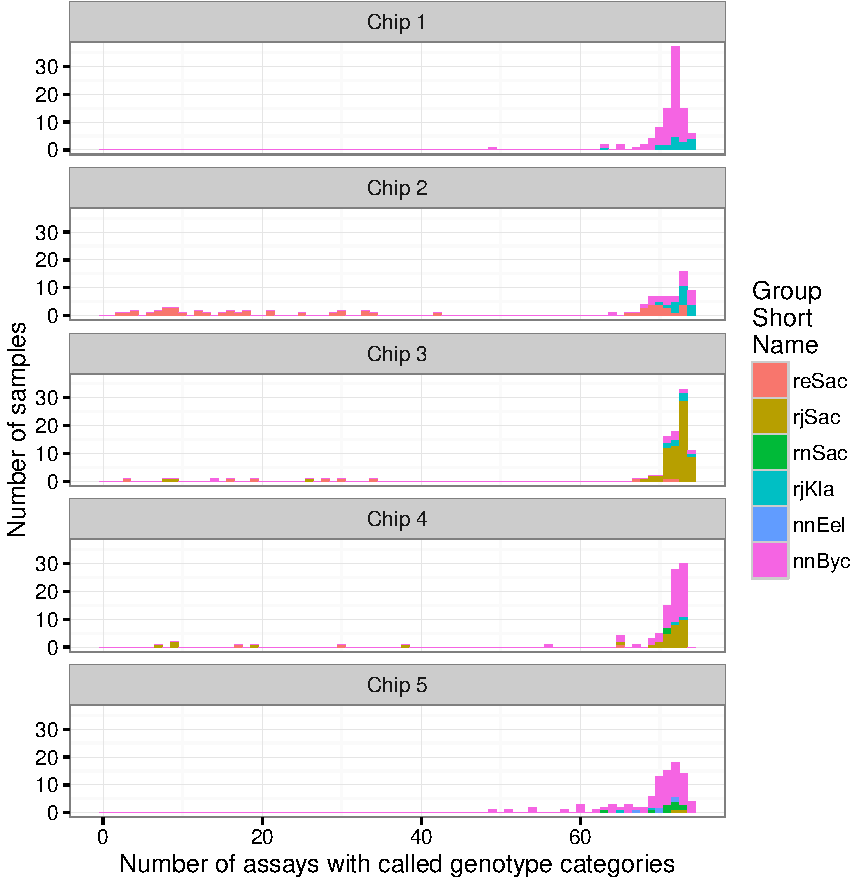
\includegraphics[width = \linewidth]{inputs/successful-assay-histogram-crop.pdf}
\end{center}
\caption{ Histogram showing the number of individuals
successfully scored for $0,\ldots, 74$ assays, on each of the chips.  Color denotes type of sample; Group Short
Names as in Table~\ref{tab:samps}.  \label{fig:success-histos}}
\end{figure}



\subsection{Analysis with {\em structure}}
The 319 individuals with 60 or more called loci were included in the clustering analysis with {\em structure}. 
The posterior probability that each 
individual originated from one of the $K$ clusters is given in Figure~\ref{fig:distruct}. 
%%%%%%
\begin{figure*}
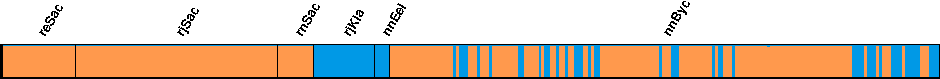
\includegraphics[width = 0.92\textwidth]{inputs/BB_ds_Clumped_TopLabel_k002r001.pdf}~\raisebox{0.96ex}{$K = 2$} \\

\includegraphics[width = 0.92\textwidth]{inputs/BB_ds_Clumped_NoLabel_k003r001.pdf}~\raisebox{0.96ex}{$K = 3$} \\

\includegraphics[width = 0.92\textwidth]{inputs/BB_ds_Clumped_NoLabel_k004r001.pdf}~\raisebox{0.96ex}{$K = 4$}
\caption{ Representative {\em distruct} \protect\citep{rosenberg2004distruct} plots of {\em structure} estimates 
of posterior probabilities of cluster membership for 319 individuals with $\geq 60$ loci. Sampling location 
codes are defined in Table~\ref{tab:samps}. Each individual is represented by a vertical bar and the amount of different colors in those
bars represents the posterior probability of cluster membership. For example, with $K=2$ each bar is either completely orange (Northern 
DPS cluster) or completely blue (Southern DPS cluster), indicating that individuals can be assigned to those clusters with effectively 
no uncertainty. For $K=3$ and $K=4$ there is more noise, indicating that a model with more than two genetic groups of green sturgeon 
is not supported by the genetic data.\label{fig:distruct}}
\end{figure*}
%%%%%
The results show unambiguously that the model for population structure that is best supported by the 
data is one with $K = 2$ genetic groups. By noting the groups to which the reference samples are assigned, it is clear 
that these two groups coincide perfectly with the Northern and Southern DPSs of green sturgeon. In addition, it is 
clear that the fish sampled from the Eel River are genetically similar to those from the Klamath River in the Northern DPS.


\subsection{Population assignment with {\em gsi\_sim}}
For performing GSI, we used data from all green sturgeon individuals, 
regardless of the number of successfully called loci. 
The known-origin reference samples from the Southern DPS (Sacramento
River) were from 150 individuals, many of which were egg samples that did not
genotype well. The known-origin reference samples from the Northern DPS (Klamath River) 
consisted of 21
fish. Consistent with the {\em structure} results, self-assignment of fish in the
baseline was very accurate. All of the fish from the Klamath were self-assigned
to the Northern DPS with posterior probabilities $> 0.999$. Likewise, all the
Sacramento fish were self-assigned to the Southern DPS except a single fish that
was called at only four loci. All of the fish in the bycatch were assigned to the
Northern or Southern DPS with posterior probabilities $> 0.999$. The poor
genotyping success with the eggs from the Sacramento River allowed us
to investigate the effect of the number of called genotypes on the confidence in
assignments (Figure~\ref{fig:sacto-self-ass}).
%%%%%%%%%%%
\begin{figure}
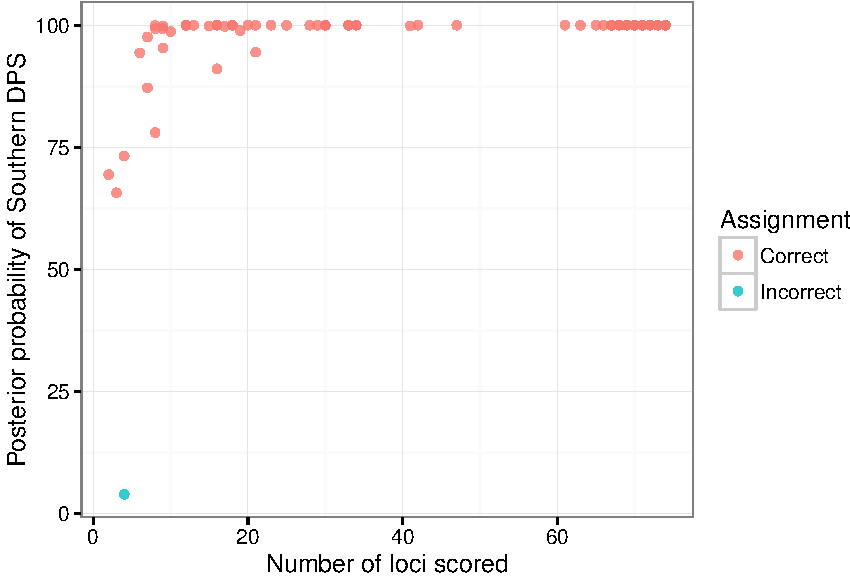
\includegraphics[width = \linewidth]{inputs/self-ass-plot-crop.pdf}
\caption{ Relationship between number of loci score and the posterior probabilities of self-assignments 
(using a leave-one-out procedure) of Sacramento River fish and eggs to
the Southern DPS.  It is remarkable that the assignments are all correct apart from one fish with only four loci scored.  \label{fig:sacto-self-ass}}
\end{figure}
%%%%%%%%%%%%%
This revealed that a correct assignment to DPS can be made
with high confidence even if as few as 10 SNPs were successfully called,
highlighting the genetic divergence between the two DPSs and indicating that the
SNP markers will be capable of correctly assigning green sturgeon to DPS even with
degraded tissues or otherwise low-quality DNA.

The green sturgeon bycatch consisted of fish that are from both the Northern and
Southern DPSs, with a greater proportion from the Southern DPS. The bycatch was
all from two fishery areas: Gulf of the Farallones, near San Francisco, CA, and around the Columbia River
plume, from Tillamook, OR to Grays Harbor, WA. The fish sampled in the southern
area were almost all from the Southern DPS, whereas those in the northern area
were a mixture of Southern and Northern DPS fish in nearly equal proportions
(Figure~\ref{fig:bycatch-map}).
\begin{figure*}
\begin{center}
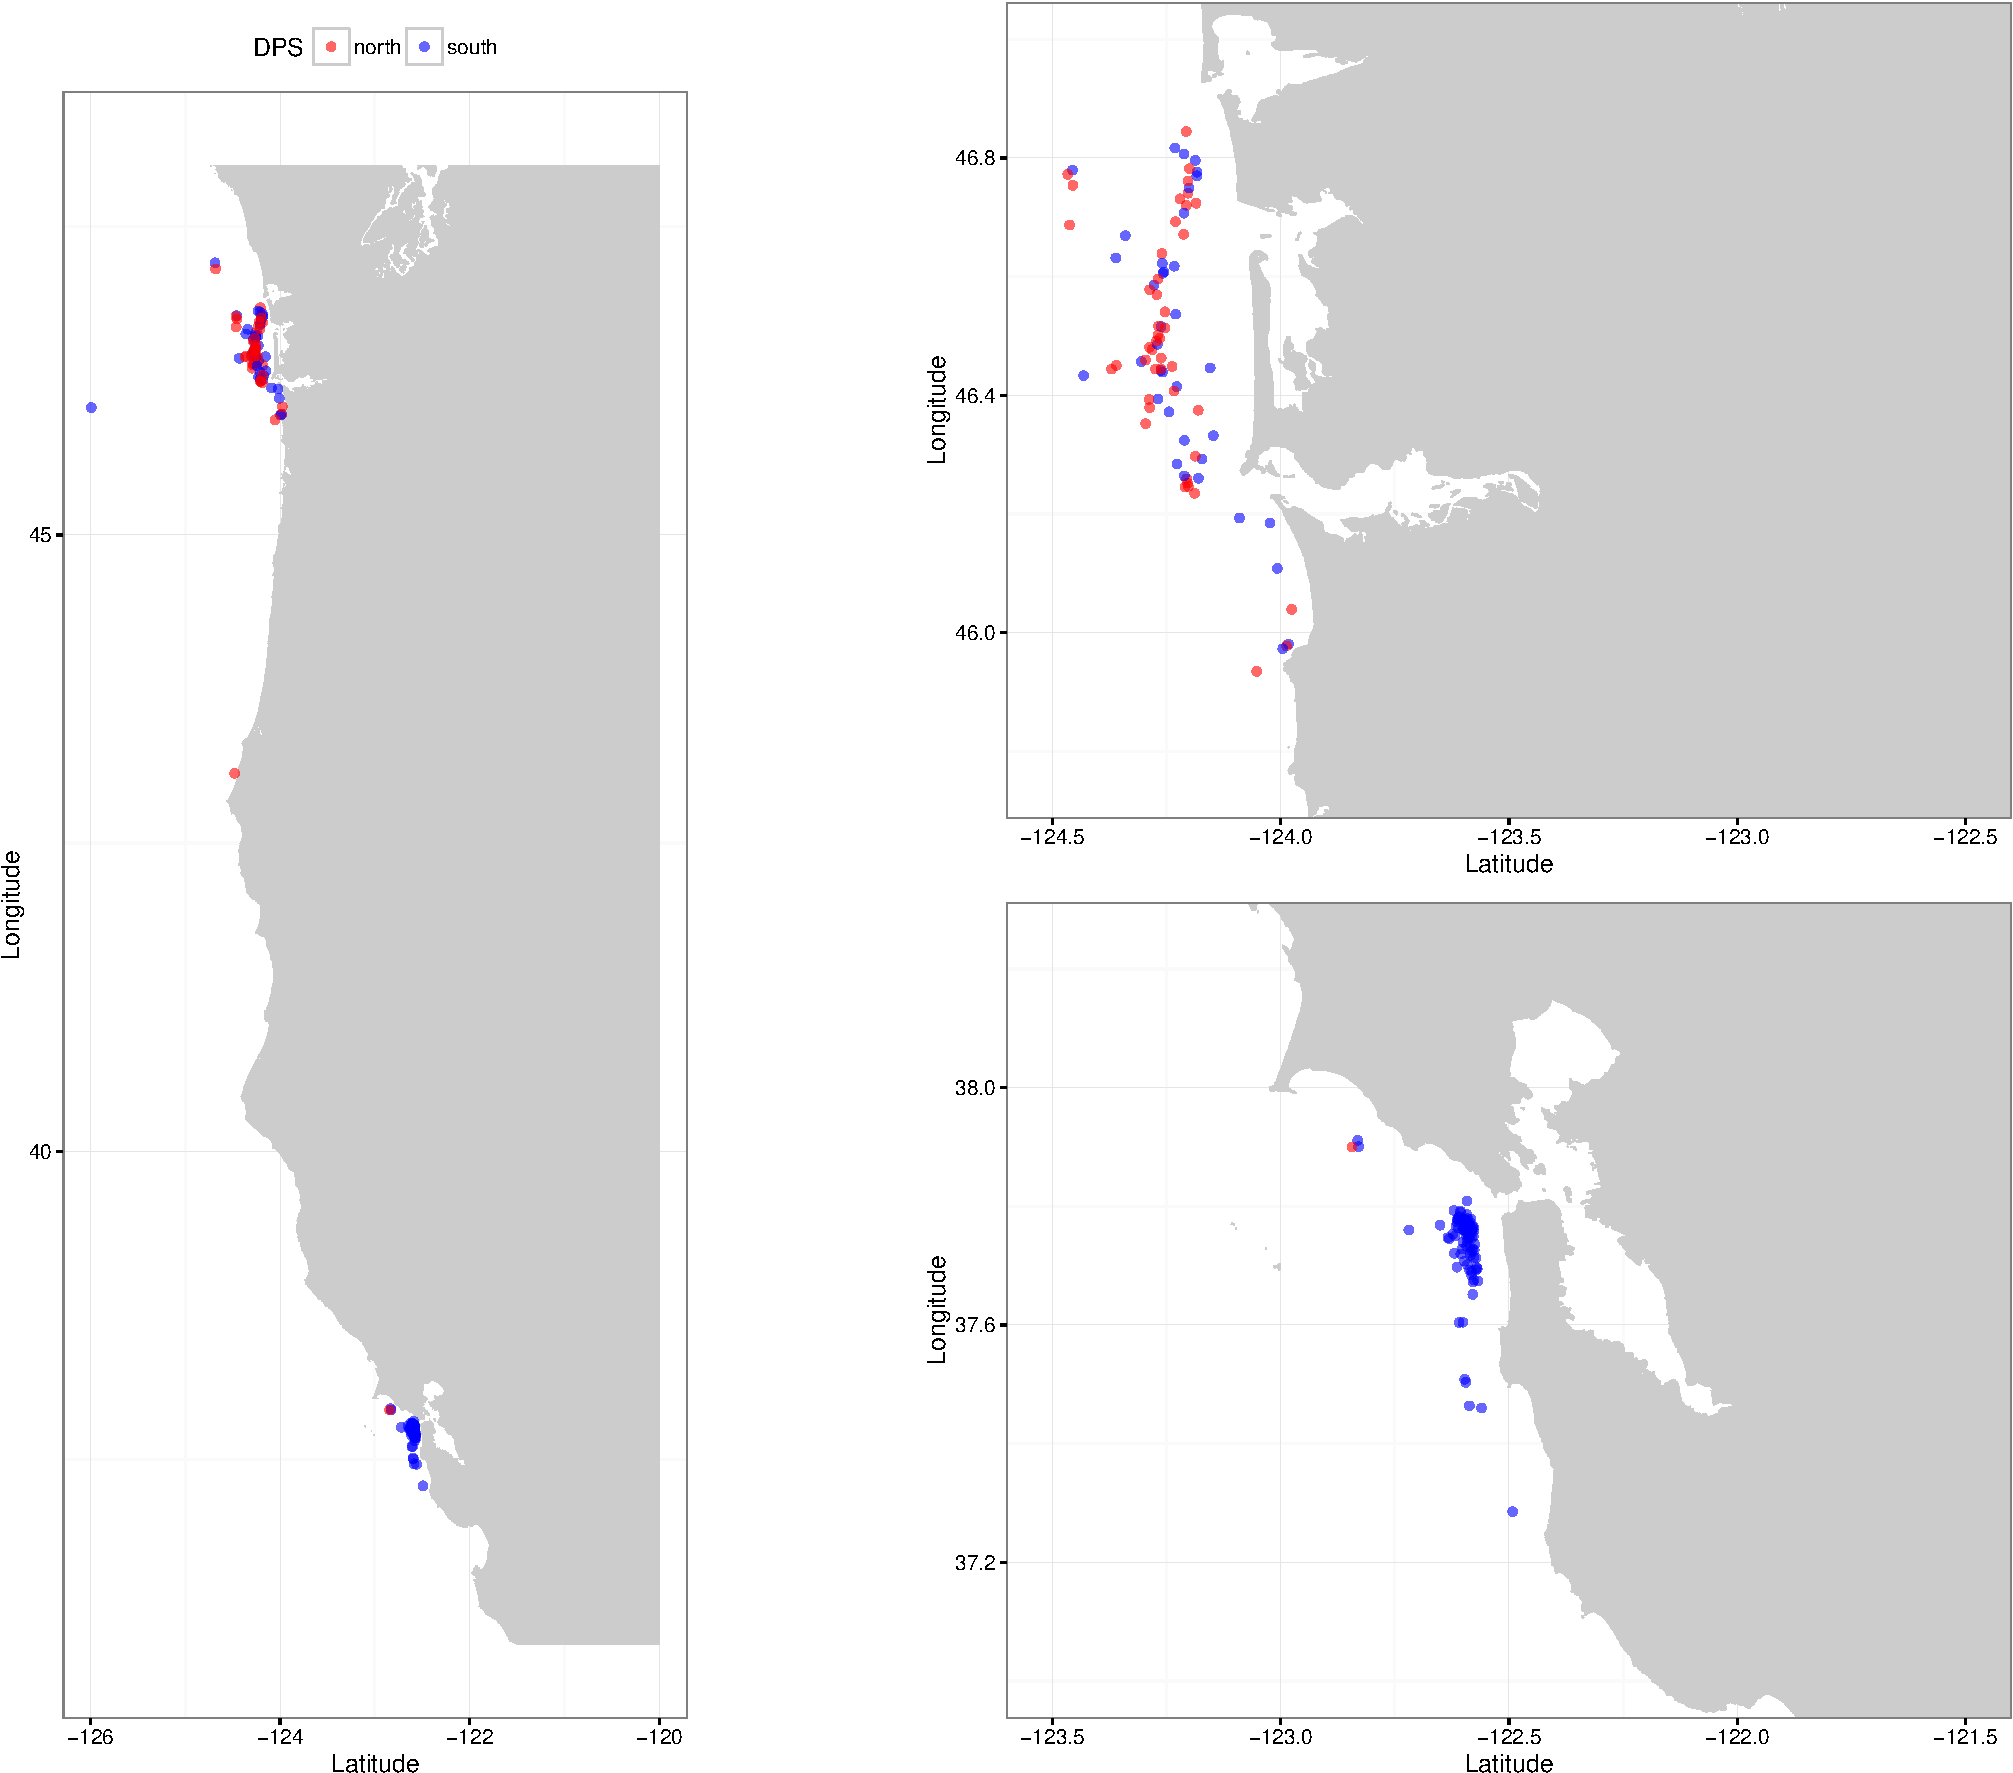
\includegraphics[width = \textwidth]{inputs/bycatch_map-crop.pdf}
\end{center}
\caption{ Location and DPS-origin of fishery bycatch samples. Left panel is a coastwide
view.  The two right panels show the Columbia Plume region (top) and the 
Gulf of the Farallones (bottom).  Each point represents one green sturgeon.  Red = Northern DPS. 
Blue = Southern DPS. }
\label{fig:bycatch-map}
\end{figure*}




\subsection{Individual identification}
Both the simulated (Fig.~\ref{fig:self-id}{\em a}) and observed (Fig.~\ref{fig:self-id}{\em b}) data 
\begin{figure*}
{\bf (a)}\\
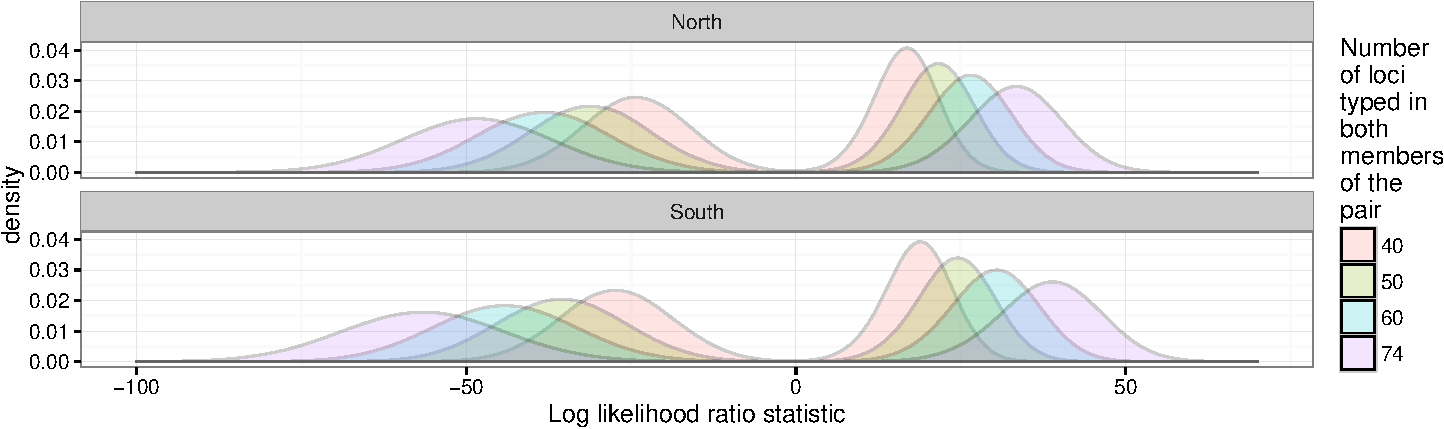
\includegraphics[width = \textwidth]{inputs/lambda_densities-crop.pdf}\\
{\bf (b)}\\
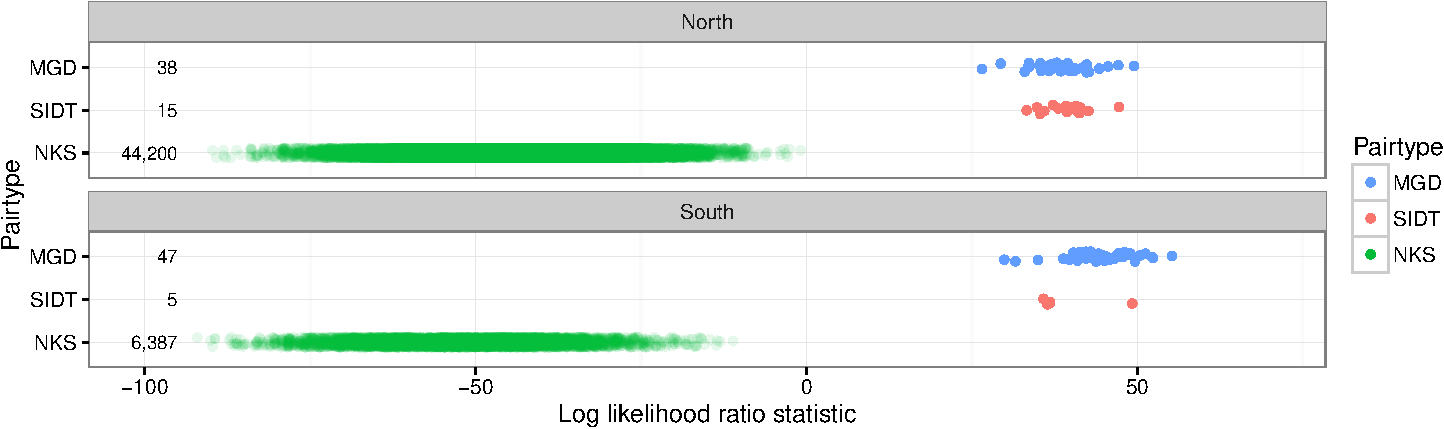
\includegraphics[width = \textwidth]{inputs/obs-self-id-logls-crop.pdf}
\caption{ Simulated ({\em a}) and observed ({\em b}) distributions of the log likelihood ratio 
statistic $\Lambda_{ij}$ for identifying samples from the same individual.  ({\em a}) The density curves on the 
left of the panel show the distribution of $\Lambda_{ij}$ for unrelated pairs (\ie $K_{ij} = \mathrm{U}$) and the 
curves on the right (having mass at values $>0$) show the distribution for samples from the same individual
($K_{ij} = \mathrm{S}$).  Different colors denote numbers of loci typed in both members of
the pair.  Curves are density estimates of $10^5$ simulated pairs for each number of loci. Simulations were done using
genotype category frequencies in the Northern and Southern DPS as indicated. $\epsilon_\ell$ was assumed to be 0.05 for
each locus. ({\em b}) Values of $\Lambda_{ij}$ observed for all pairs of individuals (from Northern or Southern DPS)
with at least 40 loci typed on both members of the pair. Different colors denote pairs of three different types: {\bf MGD}: 
``multiply genotyped DNA''---samples known to be the same sample genotyped on multiple chips; {\bf SIDT}: ``same
individual, duplicate tissue''---samples treated in the lab as completely separate, 
though they were actually two different tissues sampled from the same individual; 
{\bf NKS}: ``not known to be self''---samples that are not known {\em a priori} to 
be of the same individual. Numbers to the left of the panel indicate the total number of pairs of each of the 
three types.
\label{fig:self-id}}
\end{figure*}
revealed completely non-overlapping distributions of the likelihood ratio
statistic for pairs of samples from unique green sturgeon and pairs from the same
individual. This is true even when there is only data from 40 
of the SNP assays shared between the two genotypes.
This comparison
demonstrated unambiguous identification of samples from the same individual.




\section{Discussion}


Population genetic analysis of polyploid species has required development of an array of novel 
methods to overcome the obstacles posed by the difficulty in assigning gene copies to their 
respective loci. We report here the development of a panel of 74 SNP genotyping assays that 
target variable regions of the polyploid green sturgeon genome and a novel analytical method 
that skirts the inability to determine Mendelian relationships between gene copies by grouping 
them into ``genotype categories.'' These assays and this calling methodology provide informative 
data for several applications, including standard genetic stock identification (GSI) and 
individual (re)identification. We show that GSI with these data can accurately assign all 
individual green sturgeon to either the Northern or the Southern Distinct Population Segment (DPS) 
with extremely high confidence, even with a modest number of loci. When this GSI approach 
was applied to green sturgeon encountered as bycatch in groundfish fisheries, to categorize 
them into DPS of origin, it showed that fish sampled in the southern fishery area, the 
Gulf of the Farallones, were almost entirely from the Southern DPS, whereas those in the 
northern area, surrounding the Columbia River plume, were a nearly equal mix of fish from 
the two DPSs. Additionally, we show that green sturgeon recently encountered in the Eel River
were unambiguously 
from the Northern DPS. These fish were apparently reproducing (J. Strange \& S. Kullman, pers. comm.), 
which, if accurate, may indicate a recolonization of the Eel River, as it is recognized as
part of the Northern DPS, but its green sturgeon population was extirpated (or nearly so) in the last century \citep{adams2007population}. 
Finally, we show how these 
genetic assays allow the individual identification of green sturgeon, providing accurate 
identification of tissue samples from the same fish sampled multiple times, even when 
only a fraction of the assays are successfully genotyped. This bodes well for their 
use in forensic or other applications where DNA quality may be low. 



As green sturgeon have experienced a recent whole genome duplication, the assays described here 
interrogate more than one genomic locus and do not provide typical genotype data, 
with variants from the maternal and paternal chromosomes individually discriminated, 
but rather provide data from four gene copies (two each from both the maternal and 
paternal chromosomes). It is not possible to discriminate the different gene copies 
and assign them to locus, so we developed an heuristic method for categorizing the 
relative fluorescence intensity data from these assays into ``genotype categories.'' 
These categories are defined by clustering position on a two-dimensional graph of 
intensity of fluorescence of the two dyes from the two 
variant-specific probes. The genotype categories are intended to represent the 
five potential genotype combinations of two identical loci with the same two alleles 
present. However, we do not know the exact underlying inheritance of these variants 
and how they correspond to these genotype categories and therefore consider each 
one as an individual ``phenotypic'' character. As such, this method does not produce 
data suitable for pedigree reconstruction or other such applications where an explicit 
genetic model is necessary. Additional molecular genetic data for green sturgeon and 
methodological research will be necessary to develop markers and analytical methods 
appropriate for applications with this species that must assume Mendelian segregation 
or otherwise employ an explicit genetic model. The general approach, however, of designing 
SNP genotyping assays and then using a combination of software-generated and 
post-processing categorization, facilitated by calibration across analytical runs, 
is applicable to any polyploid species and opens up new avenues for genetic 
identification of the myriad species with multiple genome copies.

Other methods for calling the genotypes 
of tetraploid individuals using SNP assay intensity data have been recently
introduced, most notably the method implemented in the R package {\sc FitTetra} 
\citep{voorrips2011genotype}.   We applied {\sc FitTetra} to the green sturgeon data, 
but only 49 of the 96
SNPs were considered callable by the software, and upon visual inspection of the
intensity data for the {\sc FitTetra}-called genotypes, we did not have high confidence in their reproducibility. 
Futhermore, {\sc FitTetra} appears not to have a good 
mechanism for using the genotypes of individuals that have been genotyped on multiple chips to guide
the SNP selection and intensity-modeling process.  This led us to develop
our own procedure.  
It should be noted that the recommended procedure for using {\sc FitTetra} involves a 
substantial decision-making effort by the user, including empirical 
adjustment of parameters and some hand curation. Our approach does the same, but with a more visual
method, rather than using the underlying modeling framework of {\sc FitTetra}.



In summary, we described here a straight-forward and reliable method for identifying
green sturgeon from the two recognized DPSs. These SNP assays provide substantially 
better resolution than microsatellites that have been used previously for green sturgeon \citep{Israeletal2009} 
and are considerably less challenging to genotype and analyze. 
Additionally, they provide a means to unambiguously identify individuals that have been 
sampled more than once, which will be useful for the study of green sturgeon. In addition, 
the data strongly support the delineation of fish from the Klamath and Sacramento River 
basins into two separate DPSs. Further research analyzing samples from fish known to have 
originated in the Rogue River, the only other basin with substantial green sturgeon 
reproduction, will be required to determine whether these fish are appropriately 
grouped into the Northern DPS with Klamath River green sturgeon. 









\begin{acknowledgements}
We are grateful to Phaedra Doukakis, Melissa Neuman, and Susan Wang (NMFS West Coast Regional Office) for engaging us in this project with the goal of identifying green sturgeon bycatch, Toz Soto (Karuk Tribe) and Bill Poytress (US Fish and Wildlife Service) for providing samples of juvenile green sturgeon from the Klamath and Sacramento rivers, respectively, Vanessa Apkenas and Cassie Columbus (Southwest Fisheries Science Center) for assistance with laboratory analyses. Joshua Strange (Stillwater Sciences) and Stephen Kullman (Wiyot Tribe) provided samples from fish encountered in the Eel River, and observations regarding their reproductive status, and staff from the NMFS West Coast Fisheries Observer Program provided samples from fishery bycatch. Steven Lindley and Ethan Mora provided helpful comments on the manuscript.
\end{acknowledgements}
%%%%%%%%%%%%%%%% END MAIN BODY
